\chapter{Evaluation}
This chapter details how the knowledge graph is evaluated upon completion and measure implementation success.

\section{Requirements-Based Assessment}
\hspace{0.5cm} Assessing whether the requirements listed in the requirements chapter were achieved is important to measure the success of implementation. For each requirement, a description stating whether it was achieved will be provided. 

\subsection{Software Requirement Assessment}
\begin{longtable}{|p{2.25cm}|p{5.5cm}|p{5.5cm}|}

\hline
\textbf{Requirement No.} & \textbf{Software Requirement} & \textbf{Assessment}\\
\hline

1& 
Ontology must be correctly configured and input into SPARQL-Anything CONSTRUCT &
Ontology has been refined and adapted based on the needs of the project. All relationships or triples have either been derived from the provided ontology or appended to the ontology based on the dataset. \\
\hline

2&
The knowledge graph created must correctly reflect the organ dataset and follow ontology structure. &
A knowledge graph produced does reflect data from the organ dataset. More detail on the quality of the knowledge graph is in the next section. \\
\hline

3&
The dataset must be refined to ensure correct data is being input into the knowledge graph. &
Ontology creation extracted relevant parts of the provided ontology and data from the dataset usually mapped onto the ontology one-to-one, without further adjustment. \\
\hline

4&
The knowledge graph must expand on the current dataset using external links. &
Using the organ Wikidata site \cite{organwikidata} and organ MusicBrainz site \cite{organmusicbrainz}, data was added to the existing knowledge graph. Custom links based on data in the dataset were also added to the knowledge graph acting as further information. \\
\hline

5&
Knowledge graphs must be evaluated to prove correctness and validity. &
This will be evaluated in the next section: \textit{Knowledge Graph Assessment Quality} \\ 
\hline

6&
Speed of knowledge graph generation must be assessed. &
This will be assessed and evaluated in detail in the \textit{Query Scalability Assessment} section. \\ 
\hline
\caption{Software Requirement Assessment Table}
\end{longtable}

\subsection{User Requirement Assessment}

\begin{longtable}{|p{2.25cm}|p{4.5cm}|p{6.5cm}|}
\hline
\textbf{Requirement No.} & \textbf{User Requirement} & \textbf{Assessment}\\
\hline

1& 
User must be able to execute written query. &
User can download SPARQL Anything and execute given query on command line. \\
\hline

2&
User must be able to select an organ to view information on. &
User can view the codes of all available organs in the dataset they can view information on. This organ code can then be passed through command line. \\
\hline

3&
User must be able to see the knowledge graph after the query is executed. &
User can either view the knowledge graph on command line or in a .TTL file with a location and a name that they specify. \\
\hline

4&
User must be able to see relevant data in the knowledge graph. &
User can view the knowledge graph and see relevant data corresponding to the request organ. \\
\hline

5&
User must be able to view other relevant external data in the knowledge graph. &
User can view the knowledge graph as see external links as well as custom links based on the data from the requested organ. \\ 
\hline

\caption{User Requirement Assessment Table}
\end{longtable}
\vspace{-1.1cm}

\section{Knowledge Graph Quality Assessment}
\hspace{0.5cm} Assessment of knowledge graph quality is important to ensure the produced knowledge graph is valid and correct, using \cite{knowledgegraphevaulationbook} as guidance to assess knowledge graph quality. The 18 qualitative requirements detailed in \cite{evaluationpaper} are also used to assess quality. For each sections, specific details are assessed with explanations and assessment of the knowledge graph quality. 

The main three sections used to assess knowledge graph quality are: 

\vspace{-0.2cm}
\begin{itemize}
    \itemsep0em 
    \item Accuracy
    \vspace{-0.15cm}
    \item Coverage
    \vspace{-0.15cm}
    \item Succinctness
\end{itemize}
\vspace{-0.1cm}

For each section, generated knowledge graphs for five different organs will be used to measure overall quality. Organs to be tested from the dataset are: \textit{Part14\_000Brouwershaven}, \textit{Part14\_000Niezijl}, \textit{Part14\_000Folsgare}, \textit{Part14\_000GravenhageNoorderkerk} and \textit{Part14\_000Groede}. For simplicity, a random sample of five was selected from the list of organ codes and the produced knowledge graphs will represent the quality of all possible organs. Generating the knowledge graphs and assessing quality from the output files was the method employed. 

\subsection{Accuracy}
\hspace{0.5cm} "Accuracy refers to the extent to which entities and relations- encoded by nodes and edges in the graph- correctly represent real-life phenomena". \cite{knowledgegraphevaulationbook}. In this context, accuracy means the knowledge graph generated (both subjects and relationships) needs to correctly reflect the relationships between organ topics. 

There are three types of accuracy: 

\vspace{-0.2cm}
\begin{itemize}
    \itemsep0em 
\item Syntactic Accuracy.
\vspace{-0.1cm}
\item Semantic Accuracy.
\vspace{-0.1cm}
\item Timeliness.
\end{itemize}
\vspace{-0.4cm}

\subsubsection{Syntactic Accuracy}
\hspace{0.5cm} Syntactic accuracy refers to whether the data presented is valid for it's given type. \cite{knowledgegraphevaulationbook}

\noindent An example of a potential violation: 
\begin{displayquote}
    \textit{"This is an organ" would be incompatible with xsd:integer.}
\end{displayquote}

Upon assessing the produced knowledge graphs for each of the five organs, no syntactic inaccuracies were found. Due to the ontology being derived off the provided ontology and external links, all resulting knowledge graphs did not contain any syntactic inaccuracies. 

\subsubsection{Semantic Accuracy}
\hspace{0.5cm} Semantic accuracy refers to whether data values are being correctly represented in real-world context. \cite{knowledgegraphevaulationbook}

\noindent An example of a potential violation: 
\begin{displayquote}
    \textit{Date of build (for an organ) coming after today's date.}
\end{displayquote}

In regards to semantic accuracy, none of the five organs contained inaccuracies in this context. This can be explained for similar reasons regarding the lack of syntactic inaccuracies. 

\subsubsection{Timeliness}
\hspace{0.5cm} Timeliness refers to how up-to-date or relevant the knowledge graph is with the real current state of the modern world \cite{knowledgegraphevaulationbook}. This is also in line with \cite{evaluationpaper} stating that "Knowledge graph should contain the latest resources to guarantee freshness".

\noindent An example of a potential violation:
\begin{displayquote}
    \textit{Organ's location stated as "Netherlands", but has recently been moved to Portugal and the knowledge graph has not been updated.}
\end{displayquote}

In the produced knowledge graphs, violations of timeliness can occur due to the static nature of the dataset. An example of a violation may occur when the \textit{?divisionName} is no longer the organ's current disposition in real life, but data in the dataset is not up-to-date. This particular violation, will occur over time as the organ's divisions can change over time. However at the current moment in time, no timeliness violations occur in the produced knowledge graphs.

\subsection{Coverage}
\hspace{0.5cm} "Coverage refers to avoiding the omission of domain-relevant elements, which may yield incomplete results". \cite{knowledgegraphevaulationbook}. In this context, the knowledge graph must completely fill the ontology framework in all of it's nodes and edges. This is to accurately represent the entire dataset given. 

\noindent There are two types of coverage: 

\vspace{-0.2cm}
\begin{itemize}
\itemsep0em 
\item Completeness.
\vspace{-0.1cm}
\item Representativeness.
\end{itemize}
\vspace{-0.4cm}

\subsubsection{Completeness}
\hspace{0.5cm} Completeness ensures the knowledge graph is correctly filled with all the relevant information present in a particular dataset. \cite{knowledgegraphevaulationbook}. Adding contextual information of entities and from different resources \cite{evaluationpaper} is also important to ensure completeness. 

\noindent Some examples of potential violations:

\vspace{-0.1cm}
\begin{displayquote}
    \textit{- An organ classes lacking information.}
\end{displayquote}
\vspace{-0.6cm}
\begin{displayquote}
    \textit{- Important values missing for a specific organ property.}
\end{displayquote}
\vspace{-0.1cm}

With regard to the dataset coverage, most of the data in it is represented in the knowledge graph. The reason for omission of some data is related to how it can be represented in the knowledge graph without it causing confusion. For example, the specific ranges of a given organ for each keyboard or pedal is omitted due to the possible confusion it may cause when representing the keyboard and pedal ranges (\textit{?range1} and \textit{?range2}) However, this is only relevant for some data. 

Contextual information is added in the form of descriptions and custom links in all assessed knowledge graphs. The relationship \textit{oont:extraInformation}, for instance, provides context and extra detail for that specific node. 

Different resources can be seen in the five knowledge graphs such as: Wikidata links, data from the dataset and various other website links. 

\subsubsection{Representativeness}
\hspace{0.5cm} Representativeness ensures the knowledge graph does not involve any bias and does not exclude anything relevant. \cite{knowledgegraphevaulationbook}

\noindent Some examples of potential violations: 

\vspace{-0.05cm}
\begin{displayquote}
    \textit{- Under-represent organ data from other languages.}
\end{displayquote}  
\vspace{-0.4cm}
\begin{displayquote}
     \textit{- Under-represent people (e.g. organist, owner) from a particular gender, race etc. }  
\end{displayquote}

Violations regarding under-representation stems from the dataset provided. For example, the dataset is written in Dutch so organ data is limited to the Dutch language. In terms of under-representating people, anyone involved with the organ is mentioned such as: \textit{?maintainer} and \textit{?builder} so is not a violation. 

\subsection{Succinctness}
\hspace{0.5cm} "Succinctness refers to the inclusion of relevant content that is represented in a concise and intelligible manner." \cite{knowledgegraphevaulationbook}. In this context, it means the knowledge graph created should be easily understandable and to the point. 

\noindent There are two types of succinctness: 

\vspace{-0.1cm}
\begin{itemize}
    \itemsep0em 
\item Representational Conciseness.
\vspace{-0.1cm}
\item Understandability.
\end{itemize}
\vspace{-0.4cm}

\subsubsection{Representational Conciseness}
\hspace{0.5cm} Representational conciseness refers to the extent to which the knowledge graph content is compactly represented. \cite{knowledgegraphevaulationbook}. This is consistent with requirements from \cite{evaluationpaper} including: "triples should be concise" and "knowledge graph does not contain redundant triples".

\noindent An example of a potential violation: 
\vspace{-0.1cm}
\begin{displayquote}
    \textit{Containing two properties that serve the same purpose i.e.}
\end{displayquote}
\vspace{-0.5cm}
\begin{displayquote}
    \textit{- Organist}
\end{displayquote}
\vspace{-0.6cm}
\begin{displayquote}
    \textit{- Organ Player}
\end{displayquote}

\begin{figure}[H]
\begin{center}
    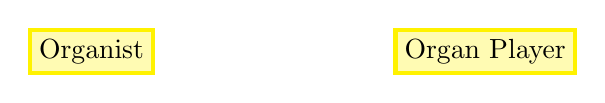
\begin{tikzpicture} [
        square/.style={draw=yellow, rectangle, ultra thick, fill=yellow!30},
        align=center,
        node distance=5cm ]
    \node[square] (q1)  {Organist};
    \node[square, right of=q1] (q2)  {Organ Player};
    \end{tikzpicture}
\end{center}
\vspace{-0.5cm}
\caption{Representational Conciseness Violation}
\end{figure}

Each knowledge graph is created with the purpose of making them concise. Creation of the ontology structure was derived and refined from the provided ontology. \textit{Figure 7.1} in the design was made specifically to represent the data in a concise manner and avoid the inclusion of redundant data. Upon assessing each organ, the produced knowledge graphs contain concise content.

\subsubsection{Understandability}
\hspace{0.5cm} Understandability refers to the need for readability and ease of understanding the knowledge graph generated. \cite{knowledgegraphevaulationbook}

\noindent An example of a potential violation: 
\vspace{-0.1cm}
\begin{displayquote}
    \textit{Using property names such as Organist1, when asked to state the name of an organist (Actual name should be used instead).}
\end{displayquote}

\begin{figure}[H]
\begin{center}
    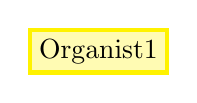
\begin{tikzpicture} [
        square/.style={draw=yellow, rectangle, ultra thick, fill=yellow!30},
        align=center,
        node distance=5cm ]
    \node[square] (q1)  {Organist1};
    \end{tikzpicture}
\end{center}
\vspace{-0.5cm}
\caption{Understandability Violation}
\end{figure}

Data in the dataset is understandable from the perspective of a Dutch reader. Given the relationships meaning of data can be easily derived. However, there are some cases in the produced knowledge graphs where nodes produce an empty string "" due to empty data in the dataset. For example, in the the variable \textit{?partition} in the ontology is often empty and out of the five tested organs, four of the partitions data is missing. 

\section{Query Scalability Assessment}
In this section, scalability of the knowledge graph will be tested. In particular, the areas being measured to assist the quantification of knowledge graph scalability are: 

\vspace{-0.1cm}
\begin{itemize}
\itemsep0cm
    \item Number of Service Calls.
    \vspace{-0.1cm}
    \item Size of Files.
    \vspace{-0.1cm}
    \item Number of Files Queried.
\end{itemize}
\vspace{-0.1cm}

For each one, measurement of scalability will be computed using the time required to execute the query on command line, which is how long it takes to generate the knowledge graph. This will make use of a command on the Windows OS called: \textit{Measure-Command} \cite{measurecommand}, which measures the time required for a command to execute. 

The same sample of five organs will be selected for knowledge graph generation and tests will be run on a 64-bit OS with Intel(R) Core(TM) i5-8265U CPU @ 1.60GHz 1.80 GHz and 8GB RAM. 

\subsection{Number of Service Calls}
\hspace{0.5cm} 


\subsection{Size of Files}
\hspace{0.5cm} 


\subsection{Number of Files Queried}
\hspace{0.5cm} 

